\section{Fundamentals}
\subsection{NTDS.DIT}
\index{Active Directory!NTDS}
\label{win:NTDS}

The NTDS.DIT file (\verb+C:\Windows\NTDS\+)  is the directory database.
It is organized into 3 key tables:
\begin{itemize}
    \item the data table:
    \item the link table:
    \item the hidden table:
\end{itemize}

In addition domain controllers also have a couple of tables that are used for
single-instance storage of ACLs and to track object quotas.

\subsubsection{Hidden table}
The hidden table is a single-row table Active Directory uses at startup to find
configuration-related information in the data table. Namely, the hidden table contains
a pointer to the domain controller’s NTDS Settings object in the data table. In addition,
there are a few other configuration-related items stored here.

\subsubsection{Data table}
The data table holds the bulk of the data in the Active Directory database. Regardless
of its class, each object in the directory, including the schema, is stored in
an individual row in this table. Each attribute defined in the schema comprises
a column in the data table.

\subsubsection{Link table}
The link table is responsible for storing the data stored in linked attributes.
Group membership is one common example of linked attribute data.



\subsection{Global Uniqque ID (GUID)}
objects have a globally unique identifier (GUID) assigned to them by the system
at creation. This 128-bit number is the Microsoft implementation of the
universally unique identifier (UUID) concept from Digital Equipment
Corporation.

The object’s GUID stays with the object until it is deleted, regardless of
whether it is renamed or moved within the directory information tree (DIT). The
ob‐ ject’s GUID will also be preserved if you move an object between domains
within a multidomain forest.

\subsection{Domain and Domain Tree}
Active Directory’s logical structure is built around the concept of domains. 

An Active Directory domain is made up of the following components:
\begin{itemize}
    \item  An X.500-based hierarchical structure of containers and objects
    \item  A DNS domain name as a unique identifier
    \item  A security service, which authenticates and authorizes any access to
        resources via accounts in the domain or trusts with other domains
    \item  Policies that dictate how functionality is restricted for users or
        machines within that domain
\end{itemize}

A domain controller (DC) can be authoritative for one and only one domain. It
is not possible to host multiple domains on a single DC.

{\bf Domain tree} is a series of domains connected together in a hierarchical
fashion, all using a contiguous naming scheme.

A domain tree is called by the name given to the root of the tree

Trees ease management and access to resources, as all the domains in a domain
tree trust one another implicitly with transitive trusts.

\subsection{Forest}
A {\bf forest} is a collection of one or more domain trees.

These domain trees share a common {\bf Schema} and {\bf Configuration
container}, and the trees as a whole are connected together through transitive
trusts.

A forest is named after the first domain that is created, also known as the
forest root domain.


\subsection{Trusts}
\label{active-directory:trust}

An Active Directory (AD) Forest is the security and administrative boundary for
objects and entities.
\href{https://social.technet.microsoft.com/wiki/contents/articles/50969.active-directory-forest-trust-attention-points.aspx}{trust}
is used to establish \verb+forest-forest+ or \verb+domain-domain+
authentication, allowing users to access resources in (or administer)  another
domain outside of the domain their account resides in. A trust  creates a link
between the authentication systems of two domains.

There are several trust types:

\begin{tabularx}{\linewidth}{|l|X|}
    \hline
Trust Type & Description \\
    \hline
Parent-child & Domains within the same forest. The child domain has a two-way
transitive trust with the parent domain. \\
    \hline
Cross-link & a trust between child domains to speed up authentication. \\
    \hline
External & A non-transitive trust between two separate domains in separate
forests which are not already joined by a forest trust. This type of trust
utilizes
\href{https://www.serverbrain.org/active-directory-2008/sid-history-and-sid-filtering.html}{SID
filtering}. \\
    \hline
Tree-root & a two-way transitive trust between a forest root domain and a new
tree root domain. They are created by design when you set up a new tree root
domain within a forest. \\
    \hline
Forest & a transitive trust between two forest root domains.\\ 
    \hline
\href{https://docs.microsoft.com/en-us/security/compass/esae-retirement}{ESAE}
    & A bastion forest used to manage Active Directory which is becoming
    obsolete\\
\end{tabularx}

\begin{figure}
  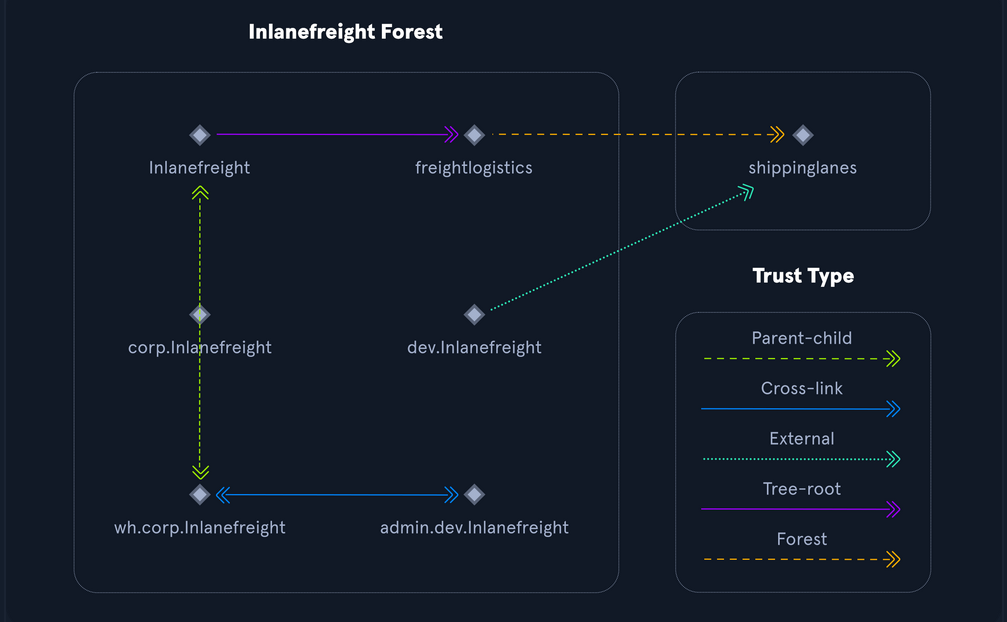
\includegraphics[width=\linewidth]{ad/knowledge/images/trusts.png}
  \caption{AD trusts}
  \label{fig:ad-trusts}
\end{figure}

Trusts can be:
\begin{itemize}
\item transitive: trust is extended to objects that the child domain trusts.
\item non-transitive: only the child domain itself is trusted.
\end{itemize}


Trusts can be set up:
\begin{itemize}
    \item bidirectional: users from both trusting domains can access resources.
    \item In a one-way trust: only users in a trusted domain can access resources in a trusting domain, not vice-versa. The direction of trust is opposite to the direction of access.
\end{itemize}

Often, domain trusts are set up improperly and provide unintended  attack
paths. Also, trusts set up for ease of use may not be reviewed  later for
potential security implications. Mergers and acquisitions can  result in
bidirectional trusts with acquired companies, unknowingly  introducing risk
into the acquiring company's environment. It is not  uncommon to be able to perform an attack such as Kerberoasting against a  domain outside the principal domain and obtain a user that has  administrative access within the principal domain.


\subsection{RootDSE and naming contexts}
\href{https://learn.microsoft.com/en-us/windows/win32/adschema/rootdse}{Active
Directory RootDSE}

Due to the distributed nature of Active Directory, it is necessary to segregate data into
partitions in order to control what is replicated. There are three predefined
naming contexts within Active Directory:
\begin{itemize}
    \item A {\bf Domain naming context} for each domain
        (\verb+DC=example,DC=com+) contains data specific to the
        domain.
    \item The {\bf Configuration naming context} for the forest
        (\verb+CN=Configuration,DC=example,DC=com+) holds data pertaining
        to the configuration of the forest (or of forest-wide applications),
        such as the objects representing naming contexts, LDAP policies, sites,
        subnets, Microsoft Exchange, \ldots
    \item The {\bf Schema naming context} for the forest
        (\verb+CN=Schema,CN=Configuration,DC=example,DC=com+) contains the set of object
        class and attribute definitions for the types of data that can be
        stored in Active Directory.
\end{itemize}

Microsoft extended the naming context concept by allowing user-defined
partitions called {\bf application partitions}. They can contain any type of
object except security principals. Application partitions are not restricted by
domain boundaries, as is the case with Domain NCs.


